\documentclass[11pt]{article}
\usepackage{graphicx}
% \graphicspath{./images/}
\textwidth=6.0in
\textheight=8.25in
\leftmargin=-0.30in
\topmargin=-0.20in
\input econfmacros.tex

\def\Title#1{\begin{center} {\Large {\bf #1} } \end{center}}

\begin{document}

\Title{NLP With Tweets}

\bigskip\bigskip

\begin{raggedright}

{\it
Ruben Gonzalez\\
Mason Speck\\
CS 4347 Section 252 - Intro to Machine Learning\\
Dr. Vangelis Metsis\\
2023-05-02
}
\bigskip\bigskip
\end{raggedright}


\section{Abstract}

% Abstract: within 150 words. What is the problem? How did you solve it? What are the final results?

This research aims to utilize natural language processing to produce a machine learning model capable of classifying posts from users of the social media website Twitter as pertaining, or not pertaining, to occurrences of natural disasters. Using a corpus of training and testing data provided by the company Figure Eight, four machine learning models were trained and optimized against already-classified posts from Twitter. After training the models, predictions were ran against a corpus of new, unclassified, and unseen Twitter posts and the accuracy of each of the models evaluated. The four models utilized were multinomial naive Bayes, random forest, logistic regression, and a multi-layer perceptron convolutional neural network (MLP). Of these models, the multinomial naive bayes model performed the best, accurately classifying 80.21\% of previously unseen and unclassified Twitter posts.

\section{Introduction}

% Introduction: describe the problem in detail. You may look up more literature and describe the problem in a broader way. Not necessarily be constrained by the description given on the Kaggle site.

% Natural disasters can occur anywhere, at any time. On a long enough timeline, the chance for a natural disaster to occur at any given location becomes a near certainty. As the frequency and severity of natural disasters increases in relation to anthropogenic climate change, the associated costs of such disasters, both in human lives and economically, will also continue to rise.

% Mitigating the effects of a nautral disaster largely relies on pre-disaster planning and resource allocation, as well as the speed at which a natural disaster can be identified and responded to. The faster a natural disaster is identified, and its severity assessed, the sooner recovery operations can begin. By analyzing the occurrence of natural diasters, their frequency, and their severity, it will be possible to better respond to these events and mitigate their impact.

\section{Methodology}

% Methodology: describe your solutions in detail. For example, the machine learning methods you used to solve the problem. The data pre-processing steps, etc.

\section{Results}

% Results: use plots and tables to format your results. And also, add necessary description words to explain the results.

After fine-tuning the parameters of each of the four models fitted against the training data, predictions were ran against previously unseen and unclassified Twitter posts. All of the models were, ostensibly, similarly accurate, with the accuracy of the models ranging approximately 4\% between the most and least-accurate models. The accuracy of the models breaks down as follows:

\begin{center}
\begin{tabular}{ |c|c| }
  Model & Accuracy\\
  \hline
  Multinomial Naive Bayes & 80.21\%\\
  Random Forest & 78.92\%\\
  Logistic Regression & 79.14\%\\
  MLP & 76.21\%\\
\end{tabular}
\end{center}

Taking into consideration that there have been, on average, 200 billion posts made on Twitter every year since 2016, any percentage of difference in accuracy is signiciant, possibly measuring in millions of correct or incorrect classification results.

Considering the dangers posed by natural disasters, and the potential for signiciantly different classification results from each model, it became important to understand how each model performed beyond a single accuracy metric. To gain insight into the characteristics of each model's performance, we generated a number of aides:
\begin{enumerate}
  \item Receiver operating characteristic curves that plot a model's true positive rate against its false positive rate.
  \item Heatmaps of a model's confusion matrix, counting and visualizing the occurrence of true positive, true negative, false positive, and false negative results.
  \item Classification reports detailing a model's most important classification metrics
\end{enumerate}

\bigskip\bigskip

% \begin{center}

\subsection{Multinomial Naive Bayes}

Multinomial naive Bayes (MNB) is a probabilistic classification algorithm. In our research, MNB was the most accurate of the four models with a weighted average accuracy of 80.21\%. As seen in the figures below, the MNB model's receiver operating characteristic (ROC) curve was steady, with an area-under-curve score of approximately 85\%. The MNB model classified the highest amount of true positive results, the third-highest amount of true negative results, the second-hightest amount of false positive results, and the least false negative results. The MNB model's values will be used as the baseline for comparisons against other models explored below.

\begin{minipage}[t]{.45\linewidth}
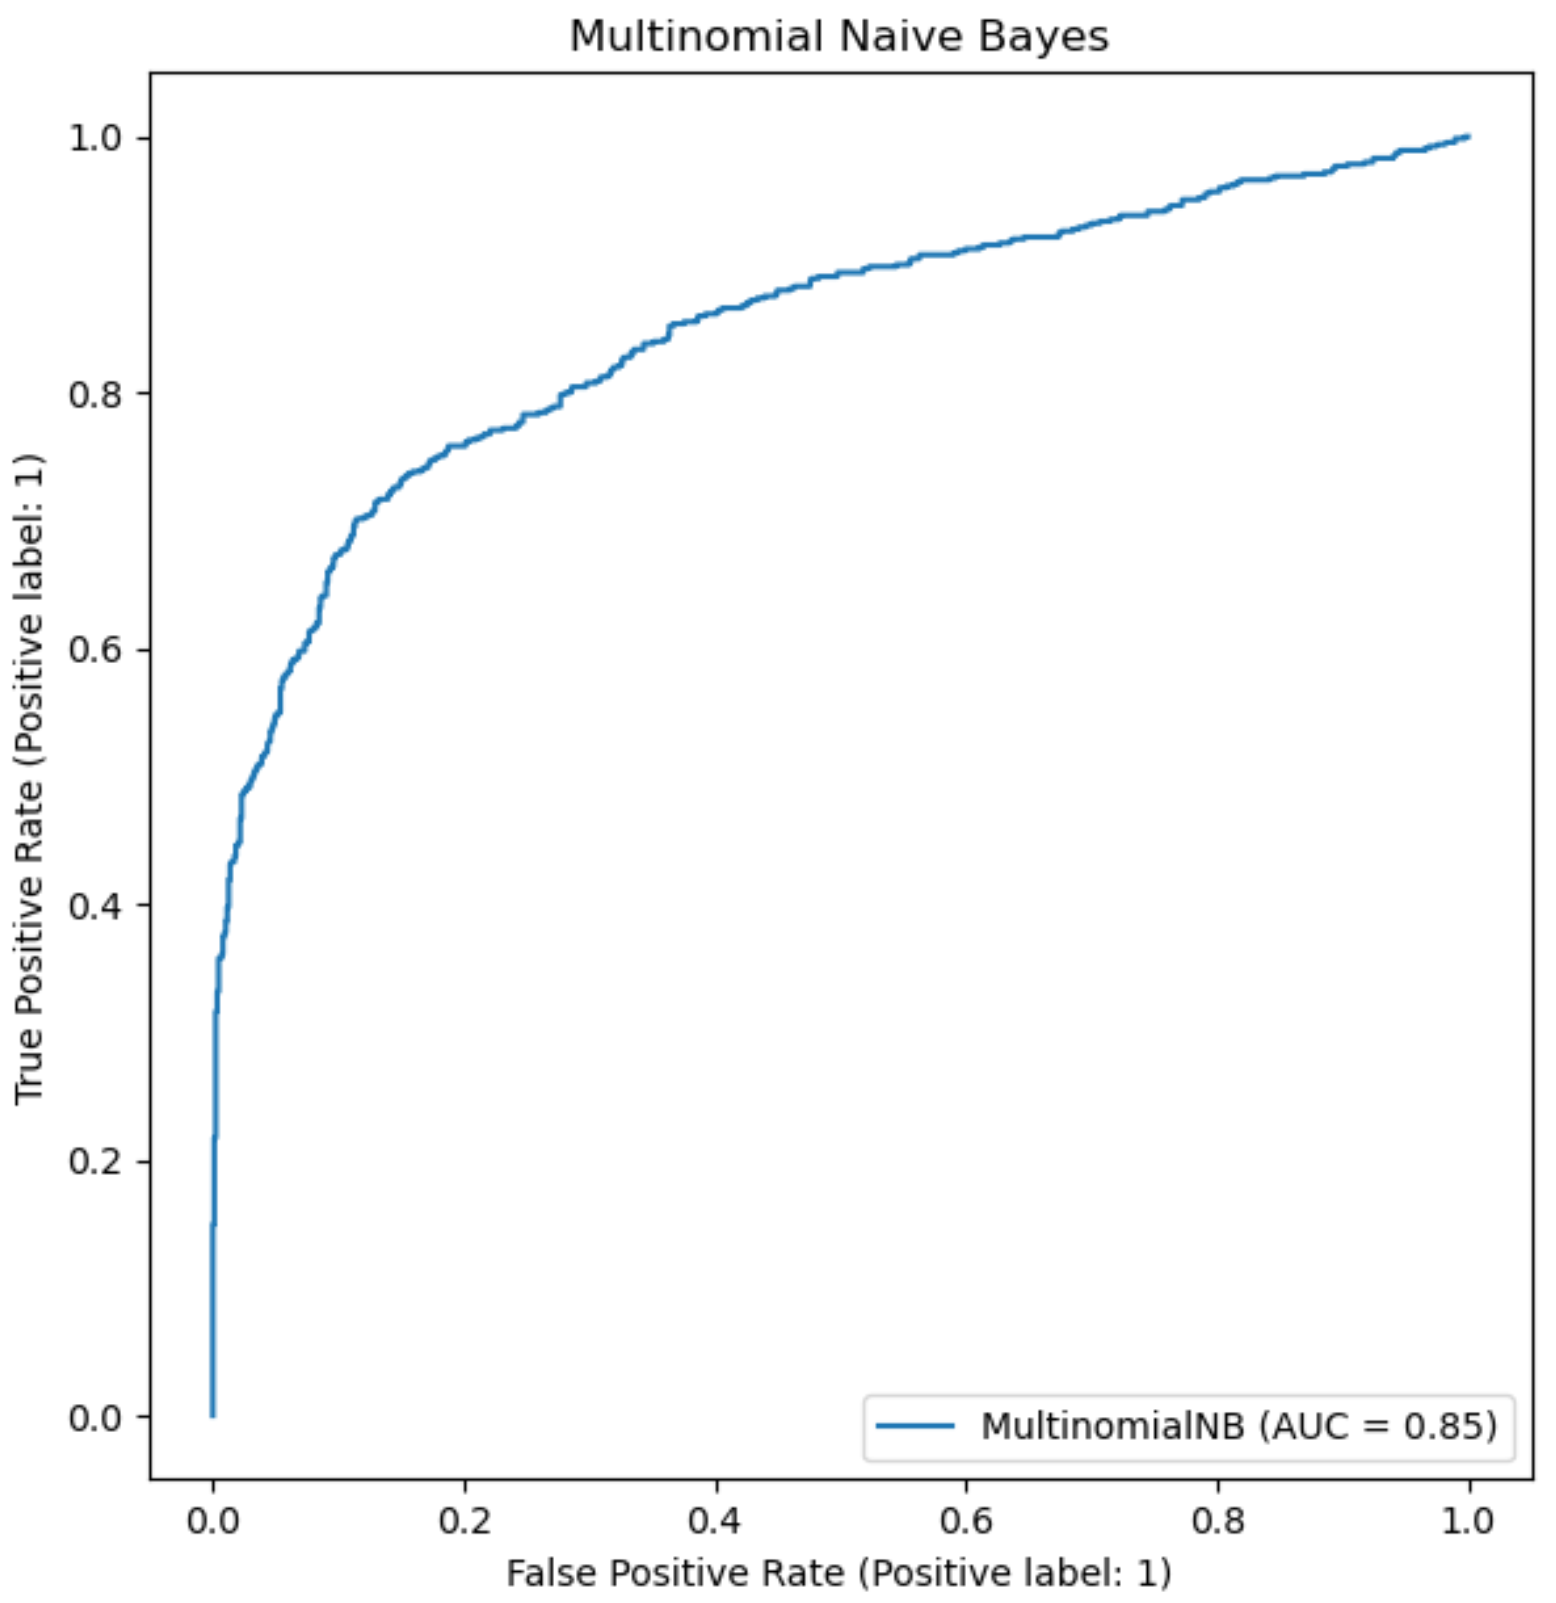
\includegraphics[width=\linewidth]{images/mnb_plot.png}
\end{minipage}\hfill
\begin{minipage}[b]{.45\linewidth}
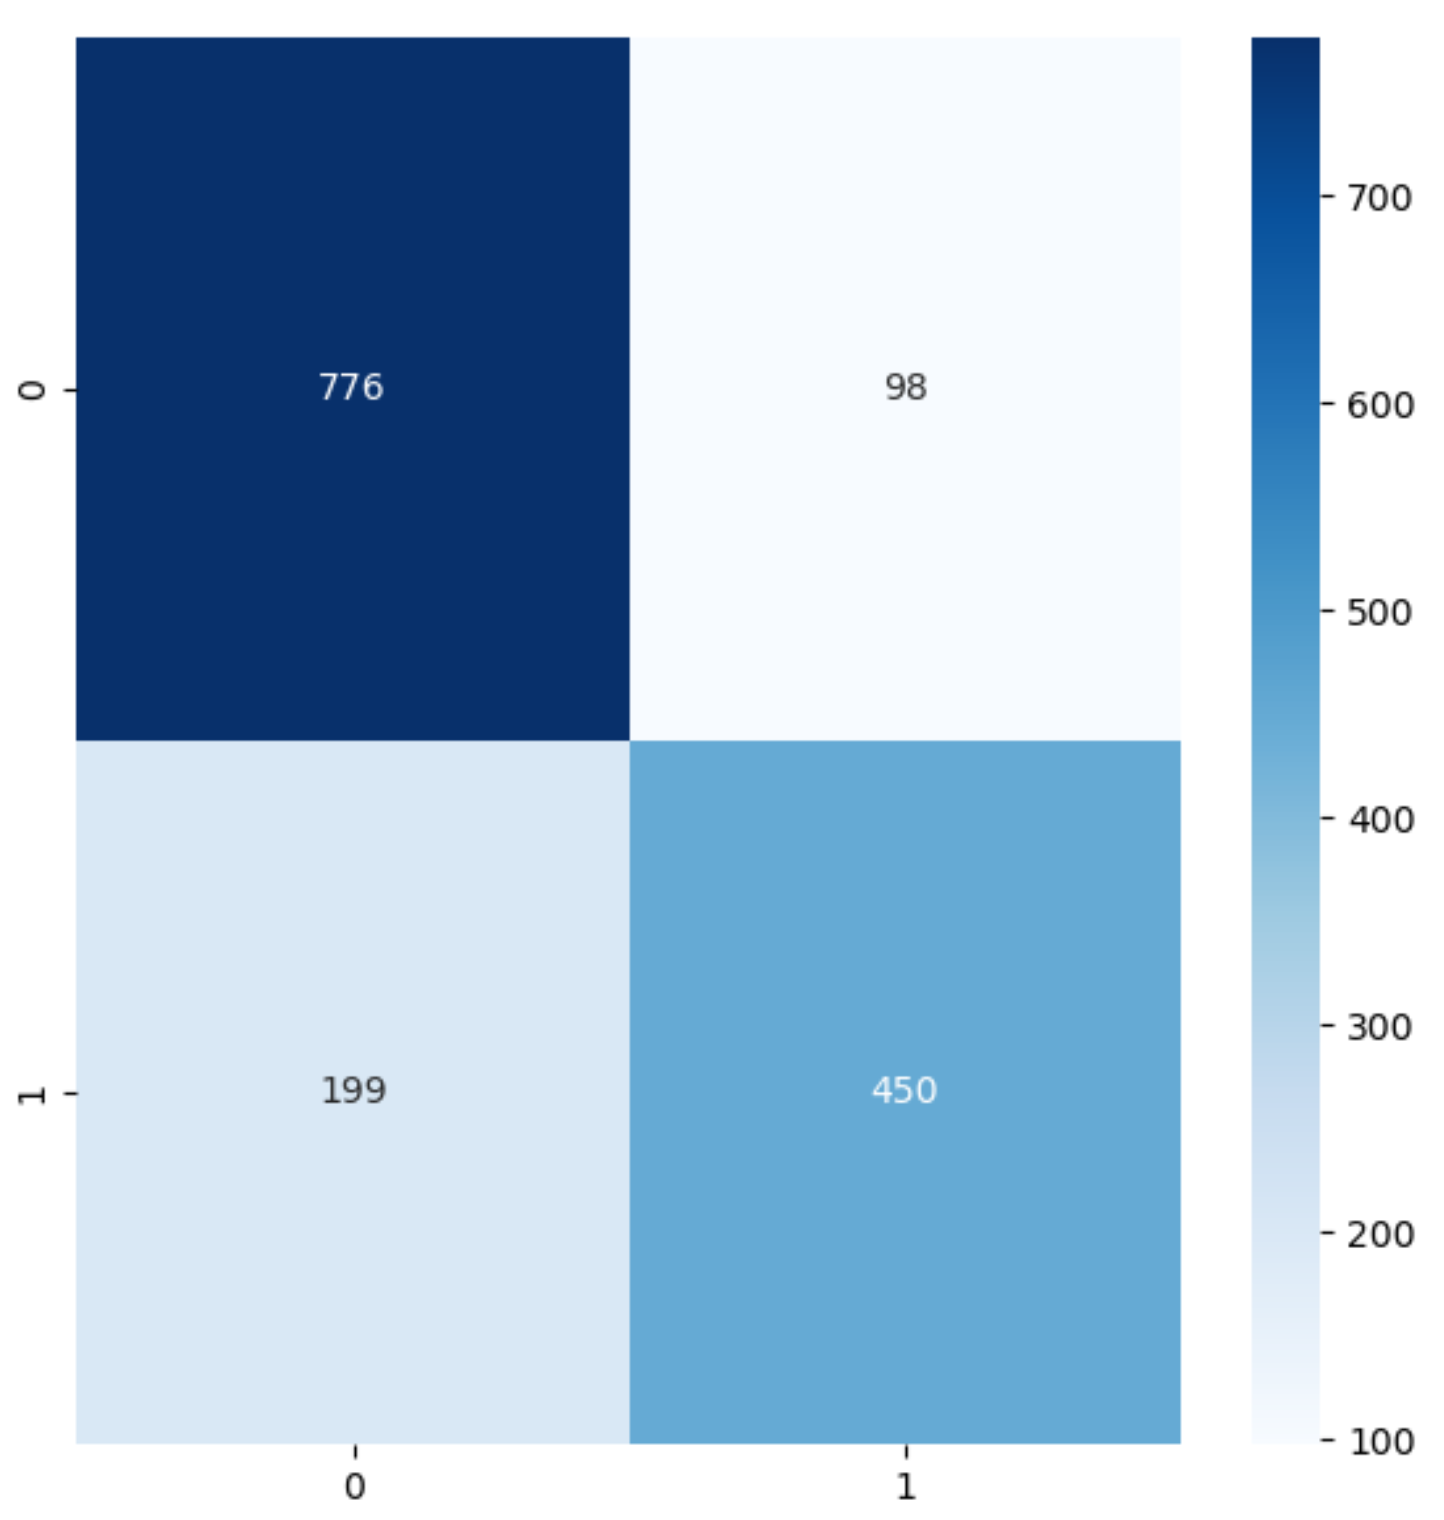
\includegraphics[width=\linewidth]{images/mnb_heatmap.png}
\end{minipage}\hfill

\subsection{Random Forest}

Random forest is a ensemble method useful for classification and regression. Random forest was the third-most accurate of the models we utilized, with a weighted average accuracy of 78.92\%. As with the MNB model, the random forest model's area-under-curve score was also approximately 85\%. Relative to MNB, the random forest model classified 90.23\% true positive results, 103.87\% true negative results, 69.39\% false positive results, and 122.11\% false negative results.

\begin{minipage}[t]{.45\linewidth}
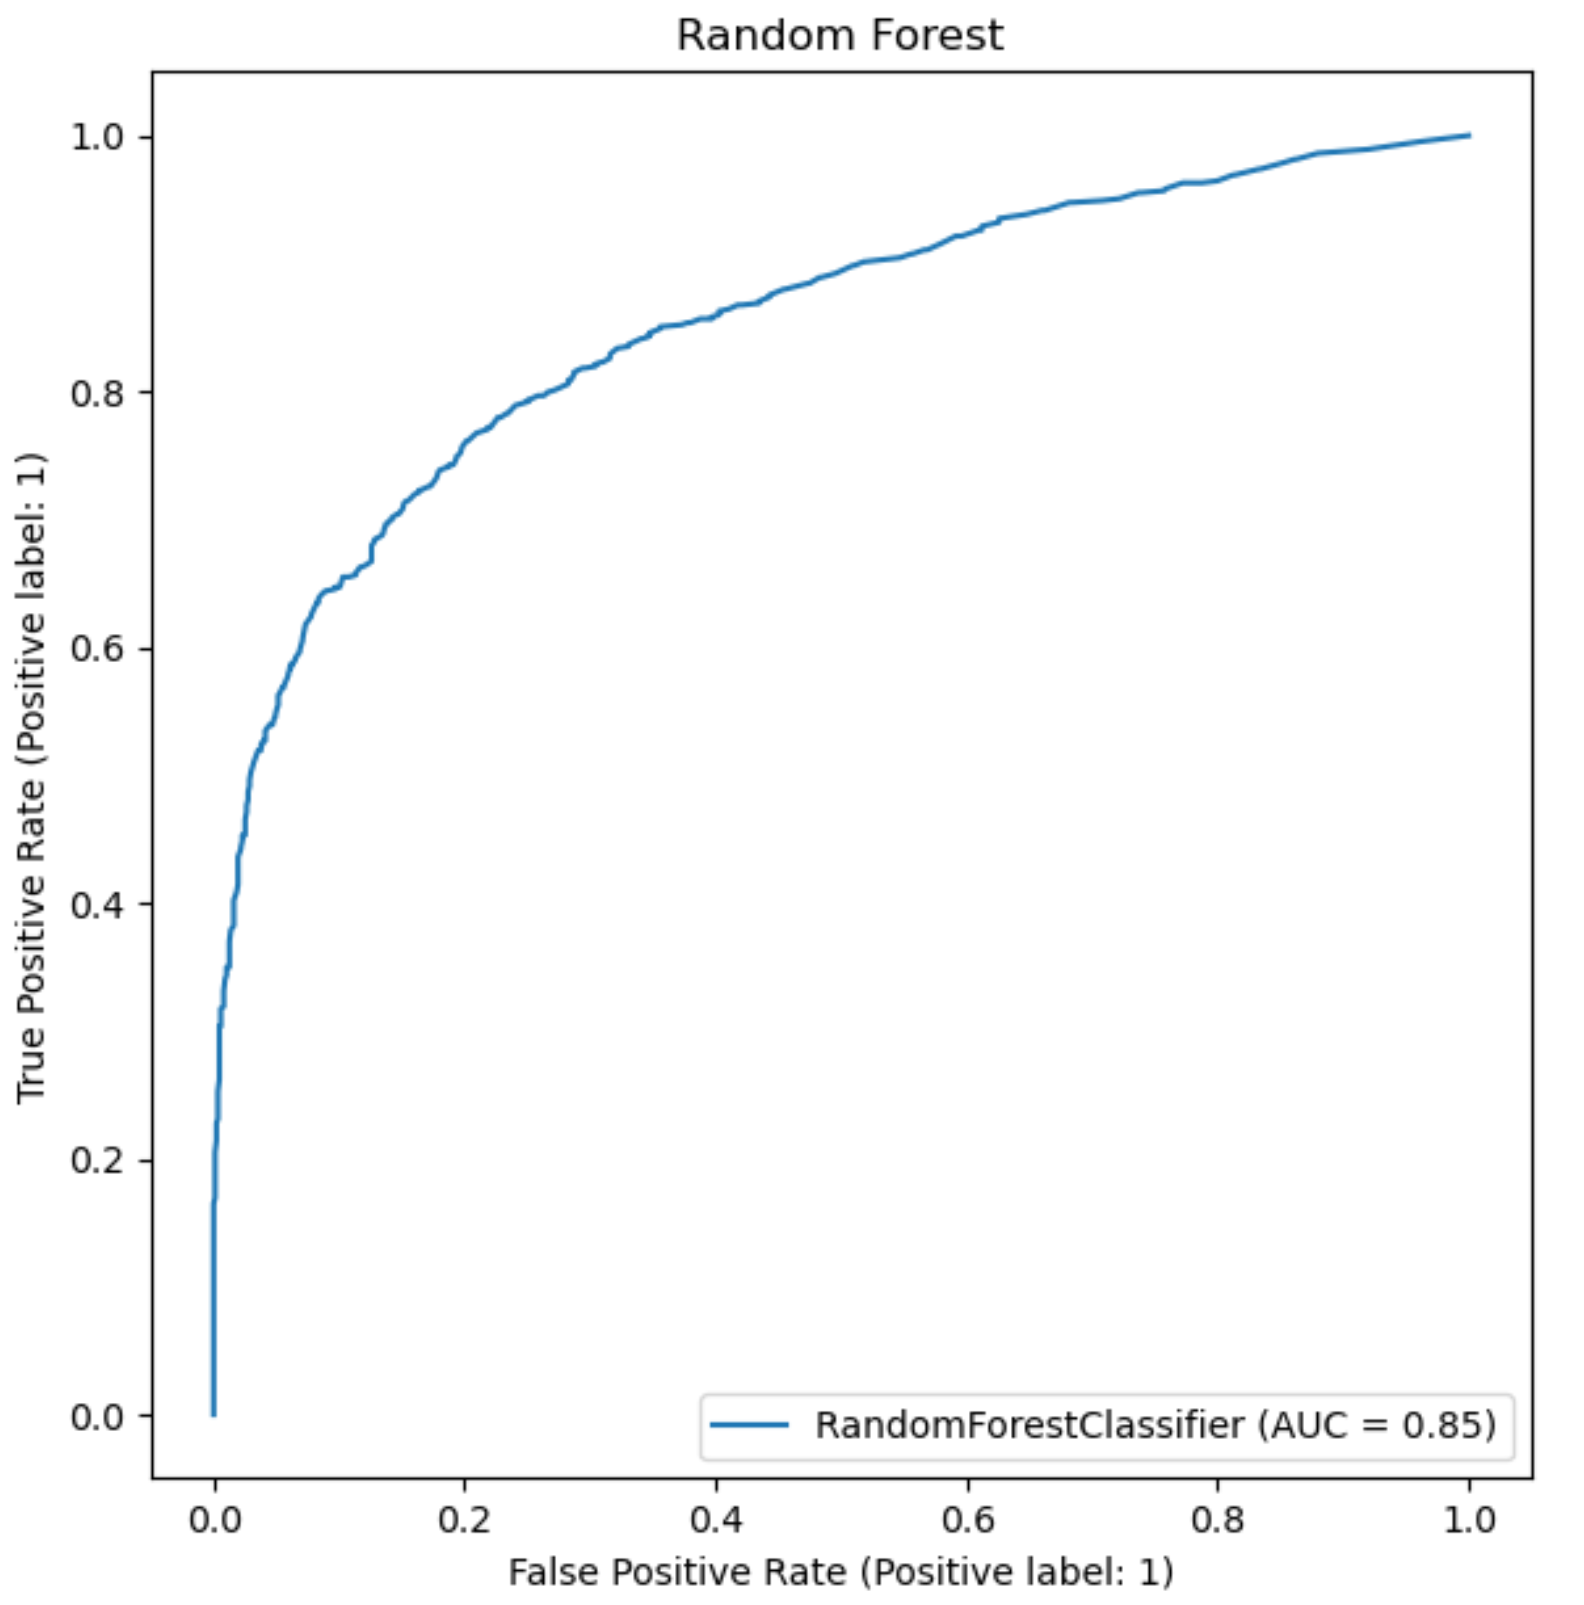
\includegraphics[width=\linewidth]{images/rf_plot.png}
\end{minipage}\hfill
\begin{minipage}[b]{.45\linewidth}
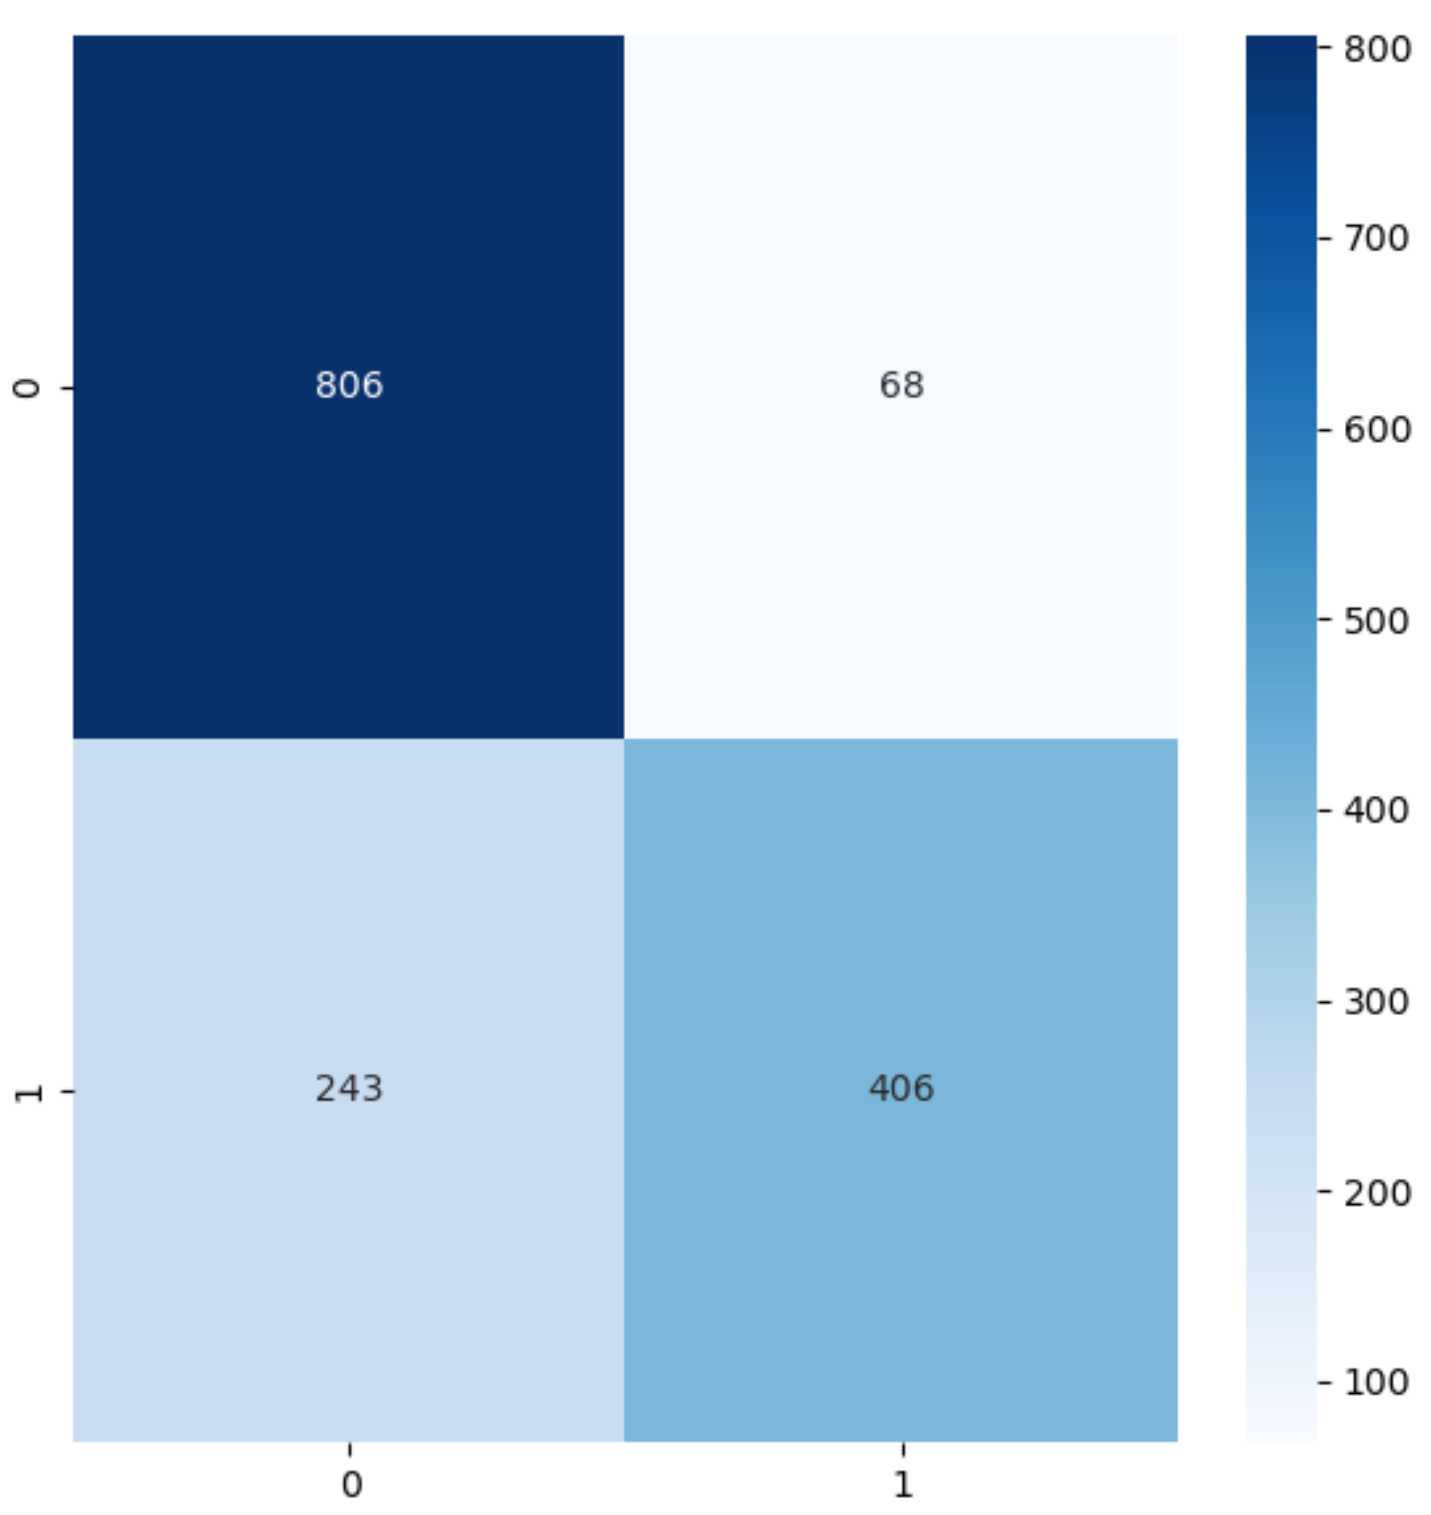
\includegraphics[width=\linewidth]{images/rf_heatmap.png}
\end{minipage}\hfill

\subsection{Logistic Regression}

Logistic regression is a regressor model that models the probabilities of linear combinations of independent variables. Logistic regression was the second-most accurate of the models in our research, with a weighted average accuracy of 79.14\%. The area-under-curve score for the logistic regression model's ROC plot was approximately 86\%. Relative to MNB, the logistic regression model classified 93.56\% true positive results, 102.10\% true negative results, 83.67\% false positive results, and 114.57\% false negative results.

\begin{minipage}[t]{.45\linewidth}
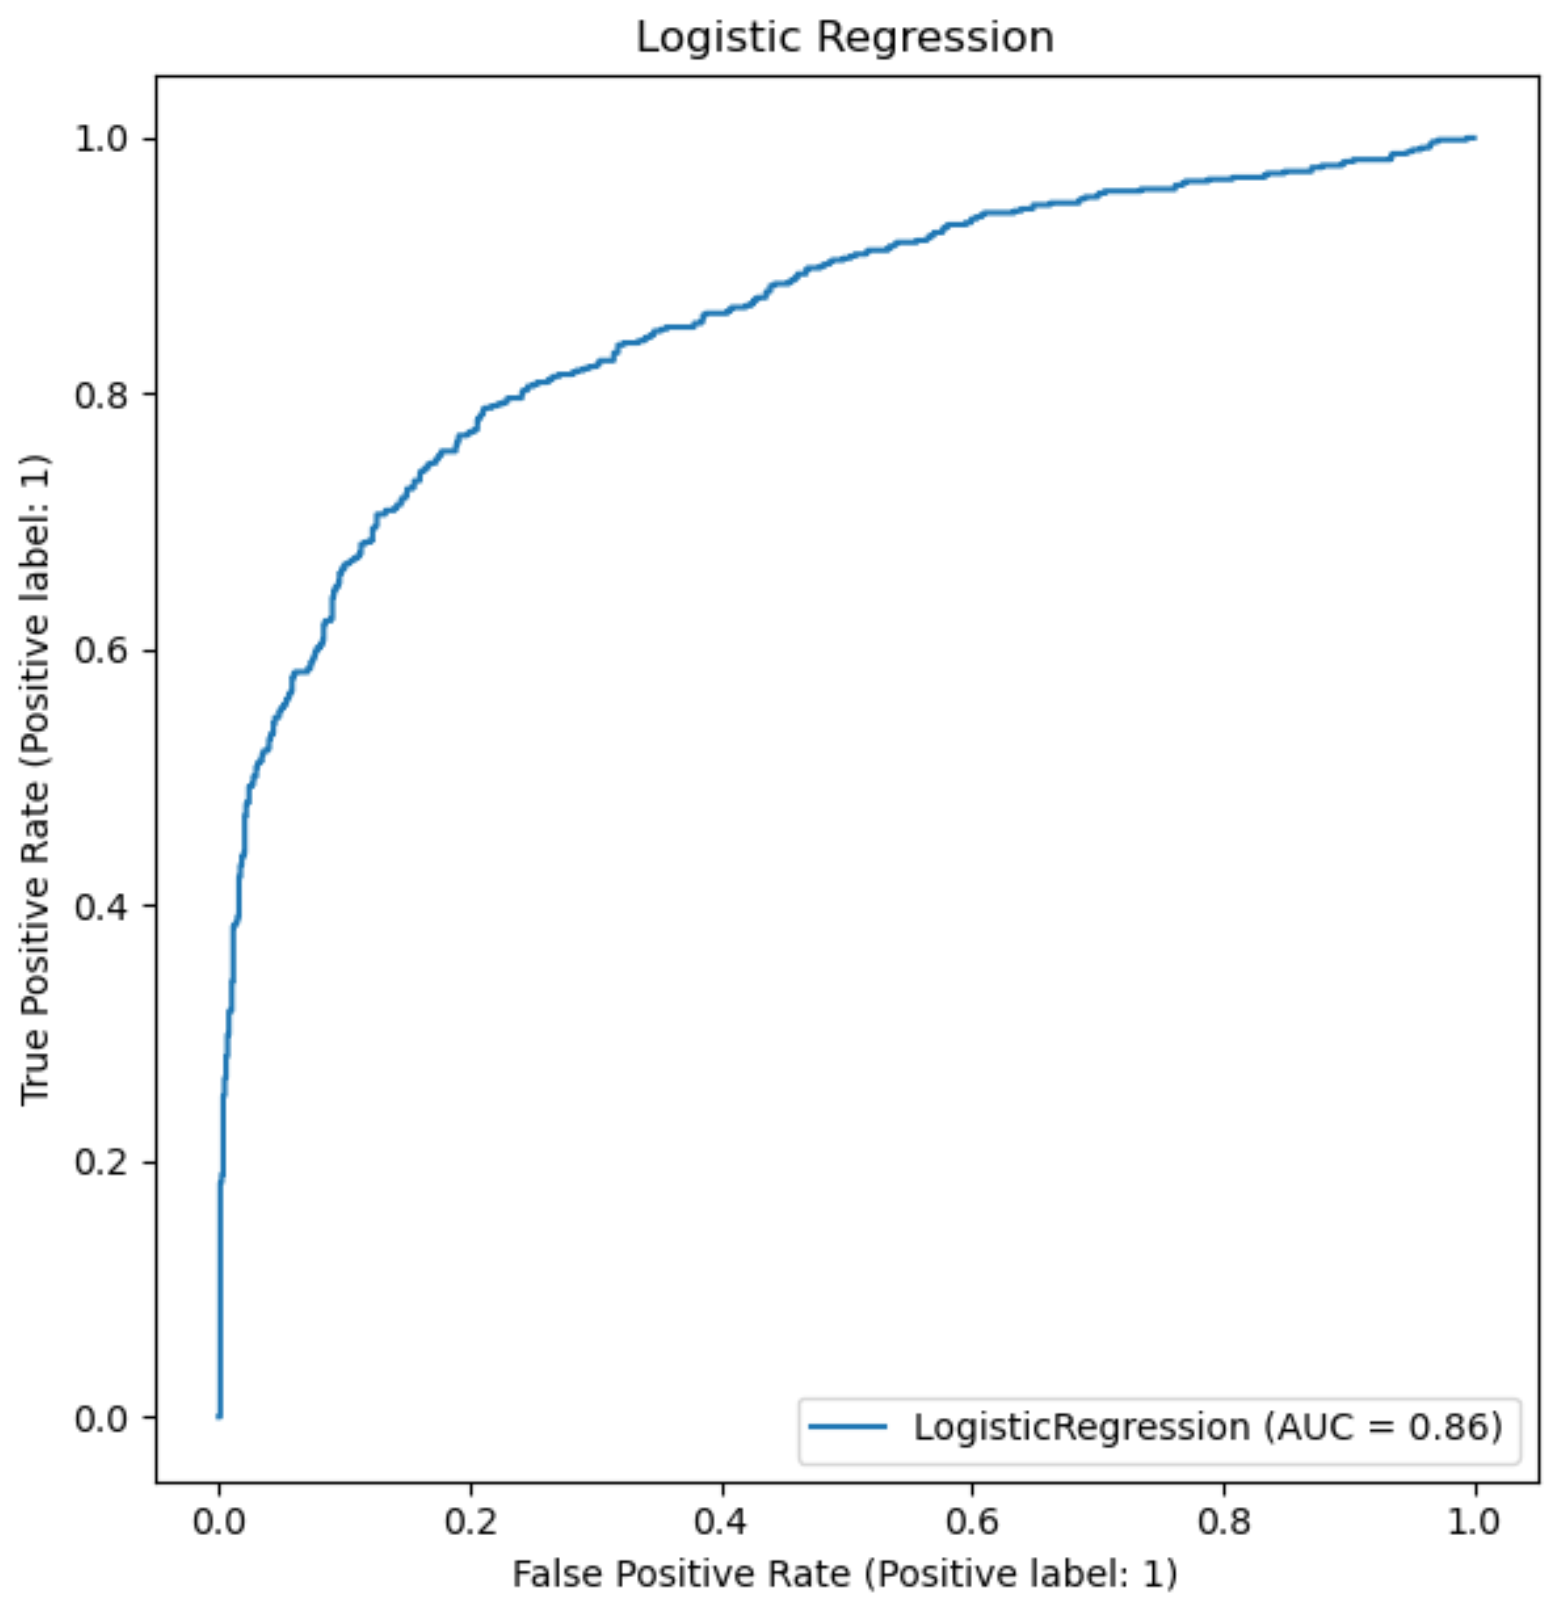
\includegraphics[width=\linewidth]{images/lr_plot.png}
\end{minipage}\hfill
\begin{minipage}[b]{.45\linewidth}
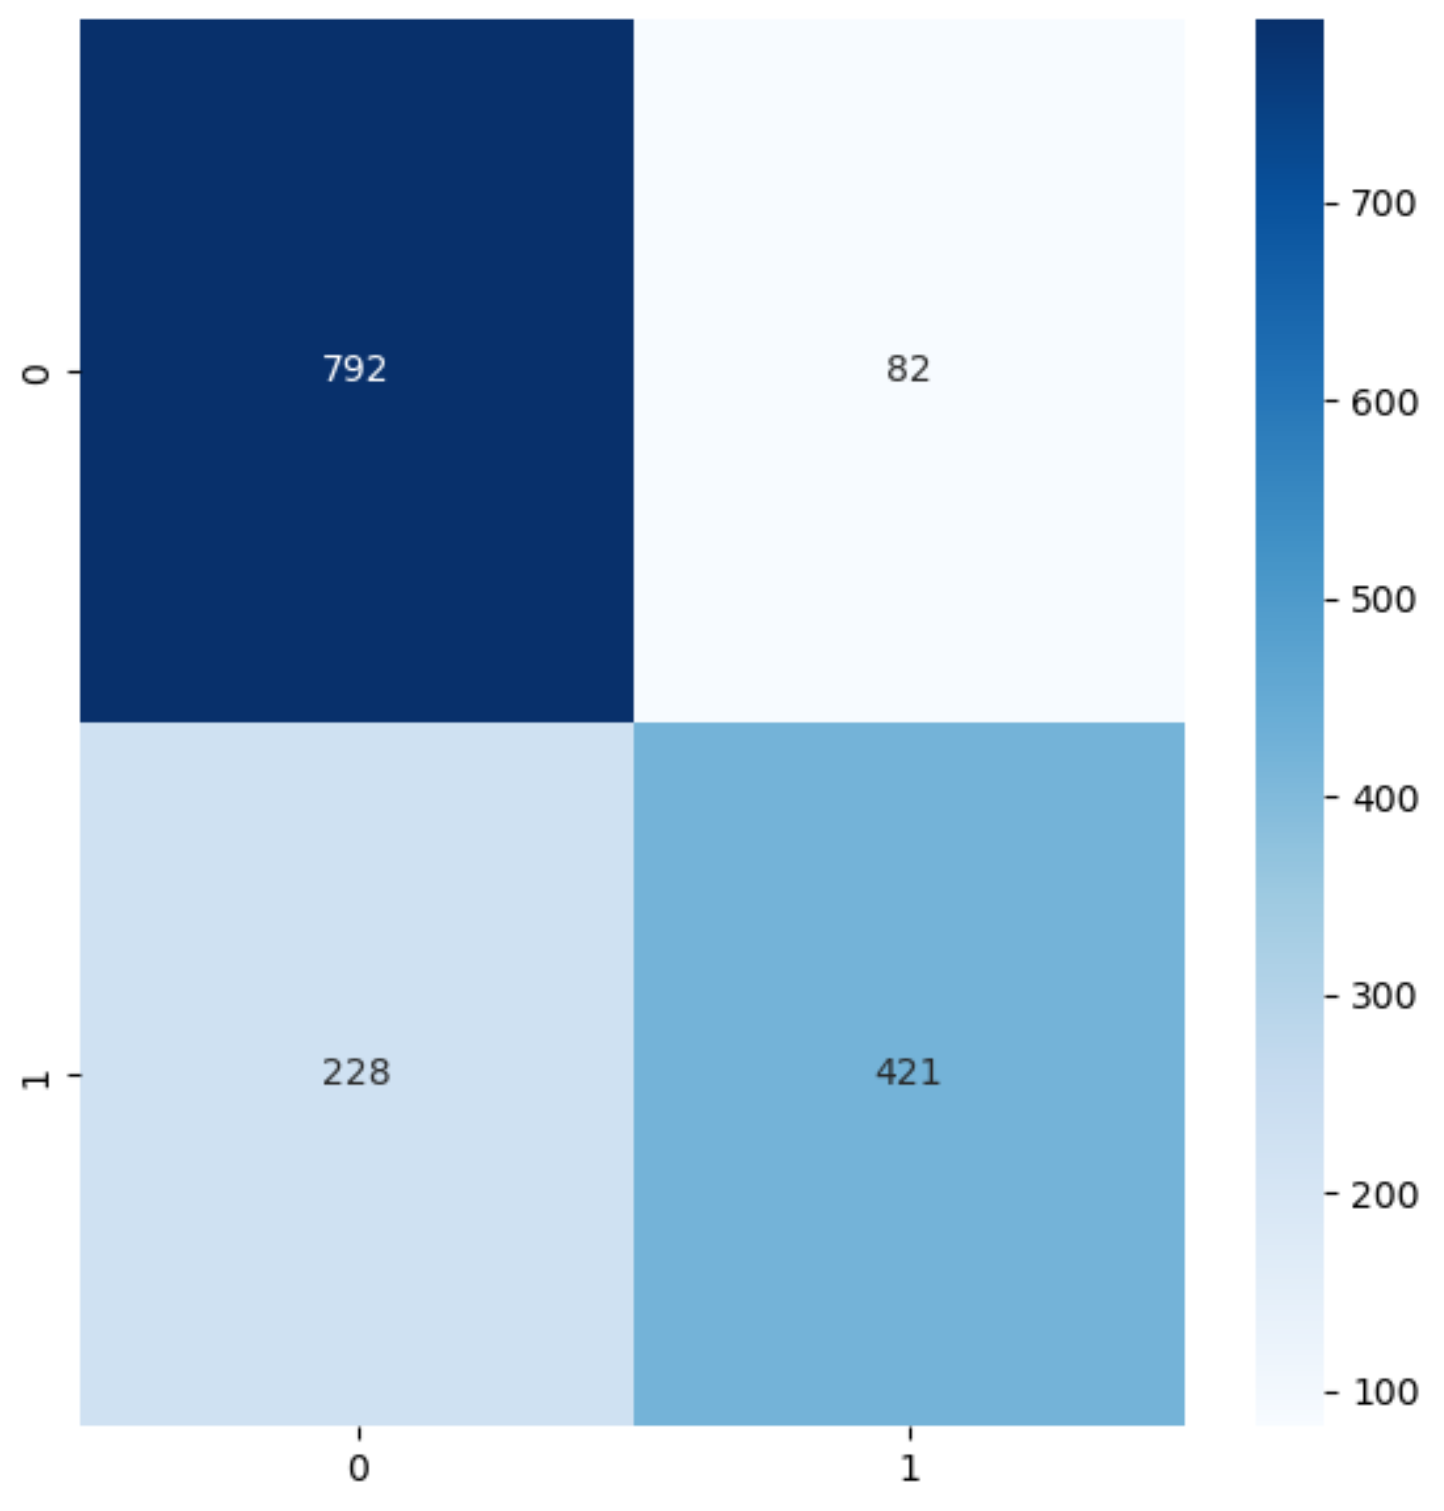
\includegraphics[width=\linewidth]{images/lr_heatmap.png}
\end{minipage}\hfill

\subsection{MLP}

The final model we used in our research was a multi-layer perceptron convolutional neural network (MLP). Compared to the other three models, the MLP model had the lowest weighted average accuracy score of 76.21\%. Relative to MNB, the MLP model classified 94.89\% true positive results, 95.10\% true negative results, 138.78\% false positive results, and 111.56\% false negative results.

\begin{minipage}[t]{.45\linewidth}
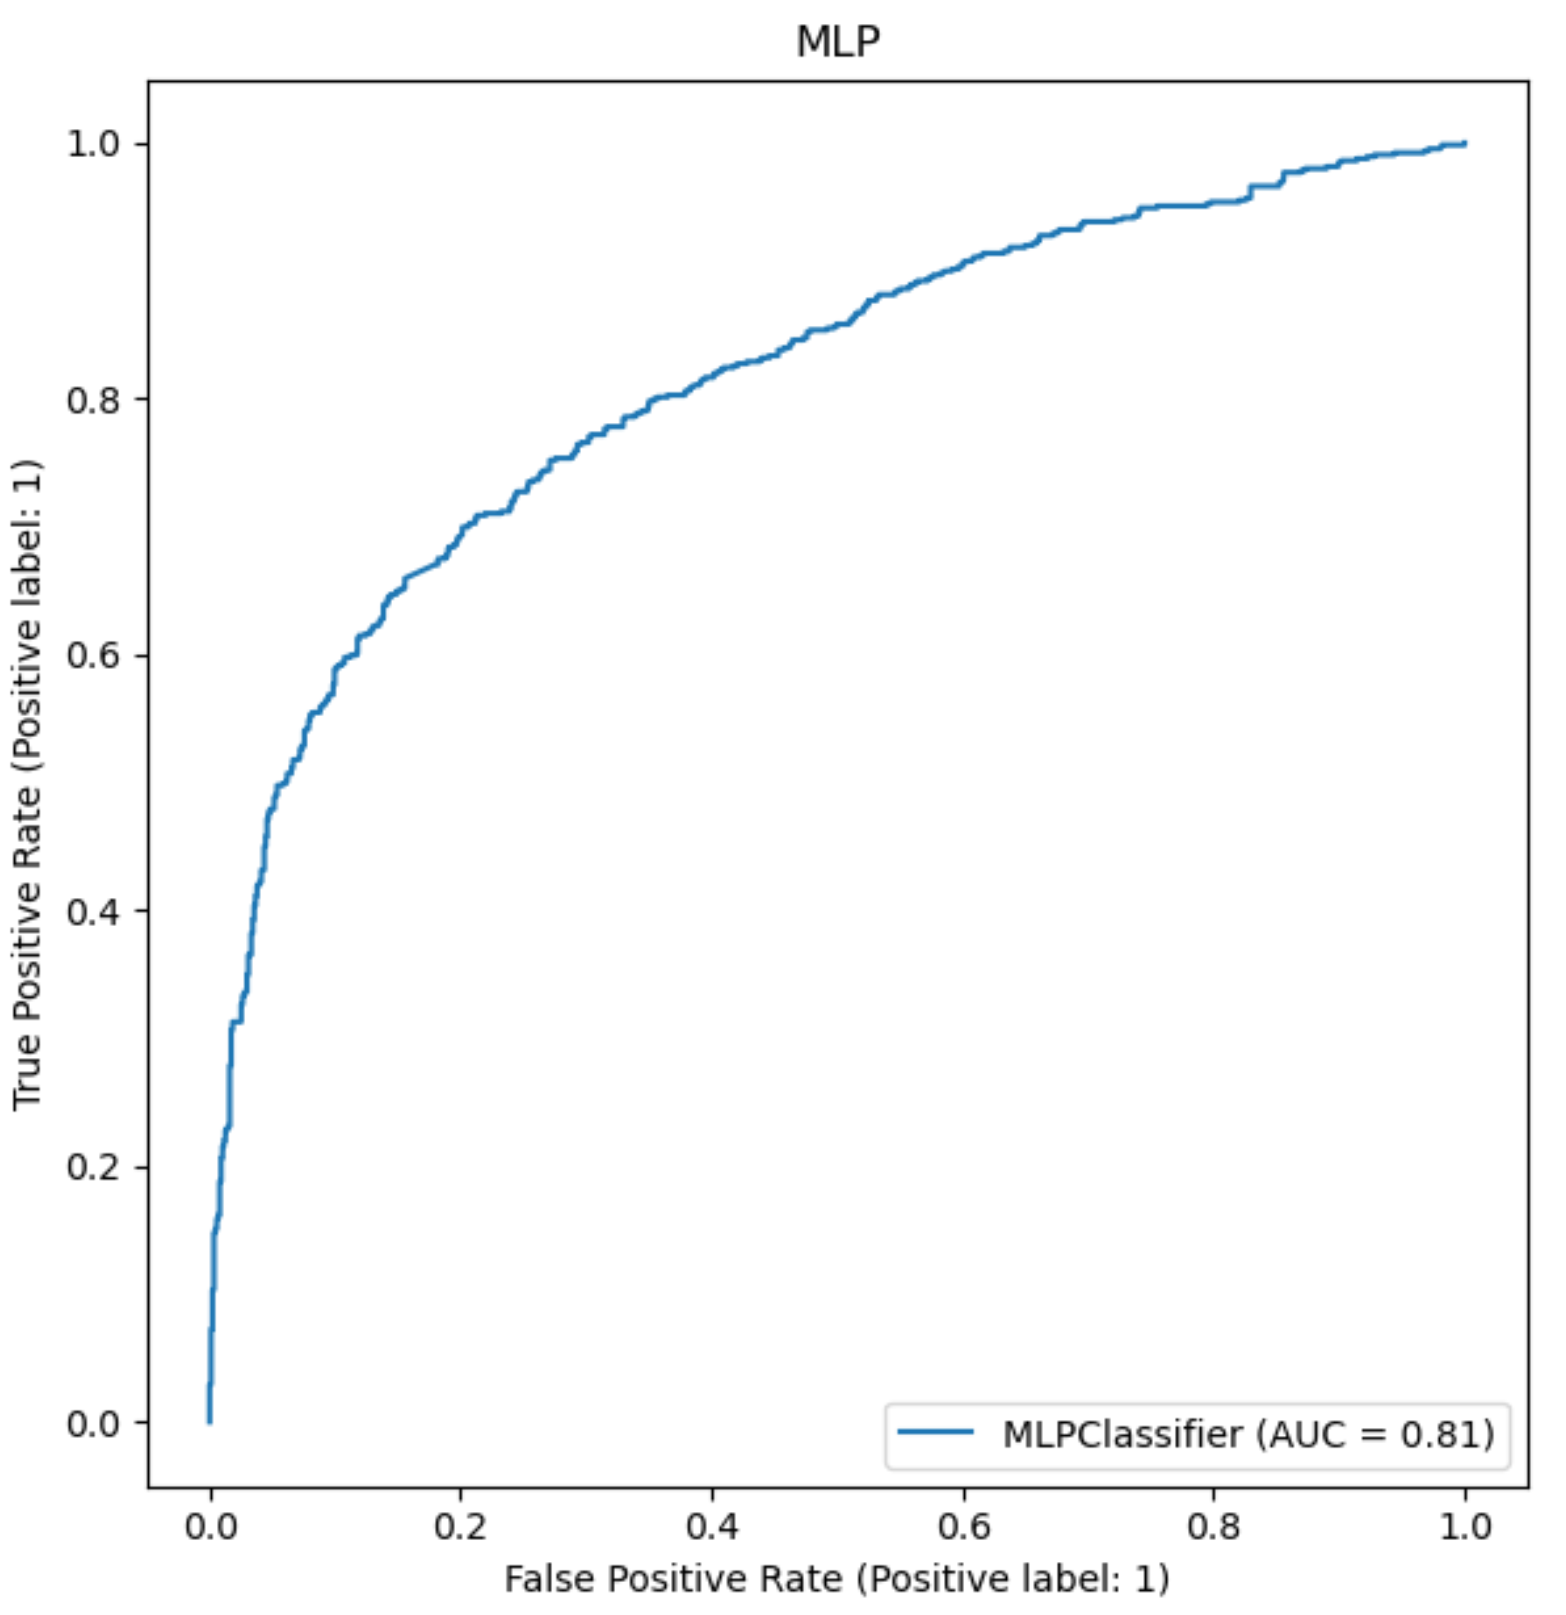
\includegraphics[width=\linewidth]{images/mlp_plot.png}
\end{minipage}\hfill
\begin{minipage}[b]{.45\linewidth}
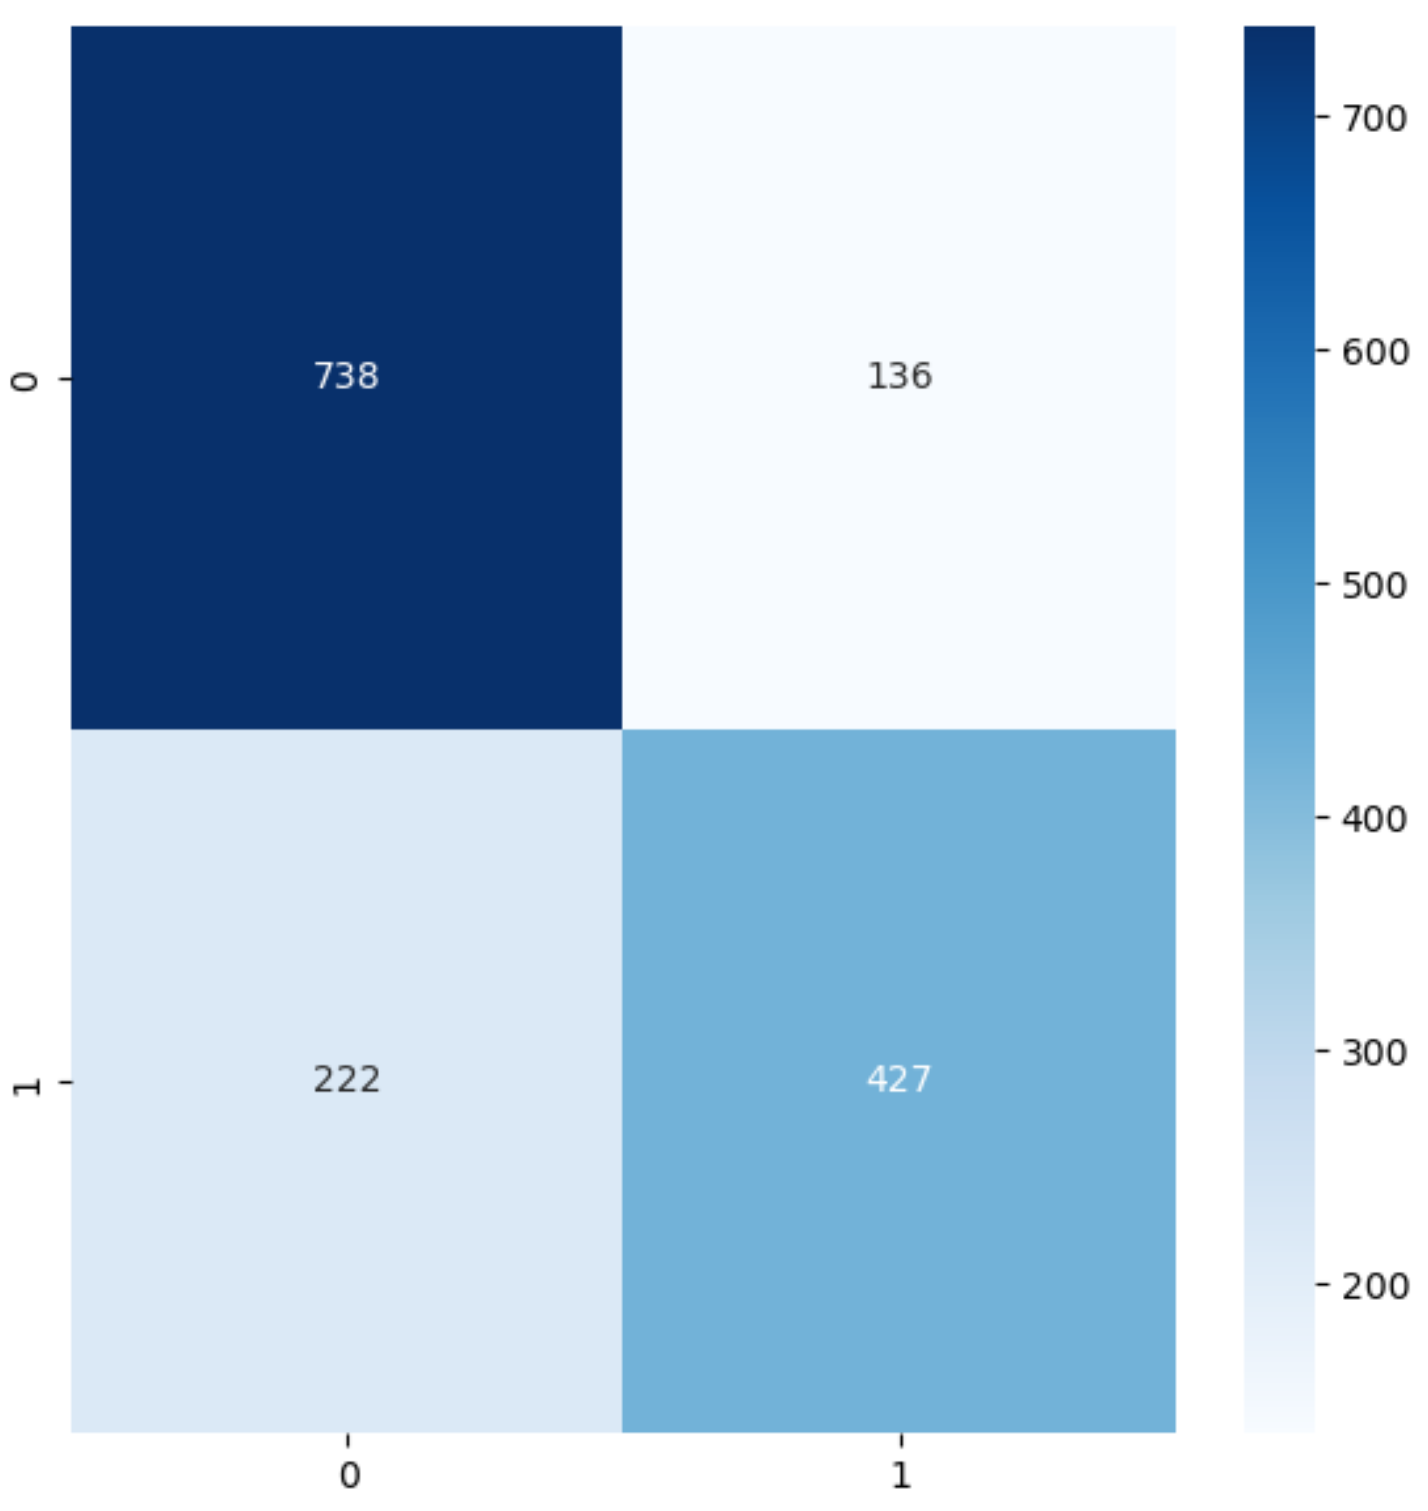
\includegraphics[width=\linewidth]{images/mlp_heatmap.png}
\end{minipage}\hfill

% \end{center}

\section{Conclusion}

% Conclusion: conclude the work.

% Isolating concentrations of results indicating natural disasters to a similar geographic area would likely increase the accuracy and usability of the system.

\end{document}